\documentclass{beamer}% тип документа

\usepackage{lingmacros}
\usepackage[utf8]{inputenc}
\usepackage{tree-dvips}
\usepackage[utf8]{inputenc}
\usepackage[T2A]{fontenc}
\usepackage[english,russian]{babel}
\usepackage[autostyle]{csquotes}
\usepackage{amssymb}
\usepackage{amsfonts}
\usepackage{amsmath}
\usepackage{color}
\usepackage{graphicx}


\usepackage{tempora} %Times New Roman alike                                     
\usepackage{newtxmath} %Times New Roman in math

\usetheme{Darmstadt}


% далее идёт преамбула
\title{Анализ жадного алгоритма для задачи 
коммивояжера на случайных входных данных}
\author{Трегубов Даниил Валерьевич МЕН-470206}

\begin{document}% начало презентации

\begin{frame}% первый слайд
\titlepage
\end{frame}


\newcommand{\algorithm}{$\mathcal{A'}$}
\newcommand{\topboundE}{$\mathcal{Z^*_{A'}}$}
\newcommand{\topboundD}{$\mathcal{D^*_{A'}}$}
\newcommand{\randomvalue}{$\mathcal{Z_{A'}}$}
\newcommand{\randomvalueE}{$E(\text{\randomvalue})$}
\newcommand{\randomvalueD}{$D(\text{\randomvalue})$}


\begin{frame}
В настоящей работе применяют следующие обозначения и сокращения.

ИБГ - Алгоритим Иди в Ближайщий Город

TSP - Travelling Salesman Problem, Задача коммивояжера

Greedy - вес маршрута коммивояжера, найденного в графе алгоритмом ИБГ

Optimal - вес оптимального маршрута коммивояжера в графе
\end{frame}

\begin{frame}% второй слайд
\frametitle{Введение}
\begin{center}
\includegraphics[width=200pt]{salesman.jpg}
\end{center}
\end{frame}

\begin{frame}% второй слайд
\frametitle{Приложения задачи коммивояжера}
\begin{enumerate}
\item<1-> Посещение n городов, населенных пунктов, точек
\item<2-> Устройство, которое может выполнять только одну работу
\item<3-> Программа для наведения интерферометра
\begin{center}
\includegraphics[width=100pt]{interf.jpg}
\end{center}
\end{enumerate}
\end{frame}

\begin{frame}
\frametitle{Математическая модель для задачи коммивояжера}
\begin{block}{Дано:}
полный взвешенный граф $G = (V,E,w)$ без петель.
\end{block}
\begin{block}{Найти:}
гамильтонов цикл минимального веса
\end{block}
\end{frame}

\begin{frame}% второй слайд
\frametitle{Постановки задачи коммивояжера}
\begin{enumerate}
\item<1-> Классическая постановка
\item<2-> Асимметричная постановка
\item<3-> Метрическая постановка
\item<4-> Max TSP
\end{enumerate}
\end{frame}

\begin{frame}% второй слайд
\frametitle{Алгоритм ИБГ}
Одним из алгоритмов, находящих некое решение за приемлемое количество операций, а именно $O(n^{2})$, где $n$ - количество вершин, является жадный алгоритм с выбором ближайшей вершины. Суть алгоритма заключается в том, что на каждом шаге мы просматриваем все непосещенные вершины в которые можно попасть из текущей вершины, и выбираем ту, расстояние до которой минимально.
\end{frame}

\begin{frame}% второй слайд
\frametitle{Пример неоптимальной работы алгоритма ИБГ}
\begin{center}
\includegraphics[width=200pt]{ris_example.png}
\end{center}
\end{frame}

\begin{frame}
\frametitle{Асимптотическая оптимальность}
Алгоритм $\mathcal{A}$ будем называть асимптотически оптимальным если существуют такие $\epsilon_n \rightarrow 0, \delta_n \rightarrow 0$ при $n \rightarrow \infty$ что применение алгоритма $\mathcal{A}$ дает значение  $\mathcal{Z_A}$, удовлетворяющее неравенству

\begin{block}{опр}
\begin{equation}\label{1}
P\{\mathcal{Z_A} \leq (1+\epsilon_n)\mathcal{Z}\}\geq 1-\delta_n
\end{equation}
\end{block}

где $\mathcal{Z_A}$ - решение, найденное алгоритмом, $\mathcal{Z}$ - минмальное решение.
Это определение при $\epsilon_n \equiv 0$ совпадает с понятием алгоритма, который почти всегда приводит к точному решению. \\

Альтернативный вариант формулы из определения:

\begin{block}{Вероятность несрабатывания}
\begin{equation}
P\{\mathcal{Z_A} > (1+\epsilon_n)\mathcal{Z}\}\leq \delta_n
\end{equation}
\end{block}
 
\end{frame}


\begin{frame}
\frametitle{Теорема Петрова}
Пусть $X_1,...,X_n$ — независимые случайные величины и
существуют положительные постоянные $g_1,...,g_n$ и $T$ такие, что для всех $0 \leq t \leq T$

\begin{equation}
\mathbb {E}e^{tX_k} \leq e^{\frac{1}{2} g_k t^{2}}
\end{equation}

Положим $S=\sum_{k=1}^{n} X_k $ и $G=\sum_{k=1}^{n} g_k $. Тогда

\begin{block}{Теорема Петрова}
\begin{equation}
P\{S > x\} \leq 
\begin{cases}
   exp (-\frac{x^{2}}{2G}), \; 0 \leq x \leq GT\\
   exp (-\frac{Tx}{2}), \; x\geq GT \\
 \end{cases}
\end{equation}
\end{block}
\end{frame}

\begin{frame}% второй слайд
\frametitle{Общее условие асимптотической оптимальности}

Найдем условия, при выполнении которых жадный алгоритм является асимптотически оптимальным, то есть
\begin{equation}\label{assymptopt}
P\{\text{\randomvalue} > (1+\epsilon_n)\mathcal{Z}\}\leq \delta_n
\end{equation}
где $\epsilon_n \rightarrow 0, \delta_n \rightarrow 0$ $n \rightarrow \infty$\\

Вес маршрута коммивояжера, полученного применением жадного алгоритма обозначим как $\text{\randomvalue}$. Он определяется формулой
\begin{equation}
\text{\randomvalue} = \sum_{k=1}^n a_{i_k i_{k+1}}
\end{equation}

Вес маршрута отпимального решения задачи обозначим как $\mathcal{Z}$. Он определяется формулой:

\begin{equation}
\mathcal{Z} = \min_{\{ \pi \}} \sum_{k=1}^n a_{i_k i_{k+1}}
\end{equation}
\end{frame}

\begin{frame}% второй слайд
Алгоритм $\mathcal{A'}$ является асимптотически оптимальным при выполнении условий $\lim\limits_{{n} \to \infty} \mathcal{I}_n = \infty $ и 
\begin{equation}
\frac{b}{a} \leq \frac{1}{\Psi(n)} min \{ \frac{1}{\gamma_n}, \frac{n}{\mathcal{I}_n} \}
\end{equation}

где:

$\gamma_n$ - корень уравнения $F(\gamma) = \frac{1}{n}$, то есть $\gamma_n = F^{-1}(\frac{1}{n})$

$\mathcal{I}_n = \int_{\gamma_n}^1 \frac{dx}{F(x)}$, 

$\Psi(n)$ - произвольная растущая от n функция, $\lim\limits_{x\to \infty} \Psi(n) = \infty $ \\



\end{frame}


\begin{frame}% второй слайд
\frametitle{Вероятностный анализ ИБГ для равномерного распределения}
Определим условия асимптотической оптимальности алгоритма $\mathcal{A}$ для случая, когда веса ребер графа $a_{ij}$ могут быть выбраны равновероятно из отрезка [a,b], a>0.

\textbf{Теорема 2}

Если элементы $a_{ij}$ матрицы А принимают значения равновероятно из отрезка [a,b], то алгоритм $\mathcal{A}$ является асимптотически оптимальным при выполнении следующего условия:
\begin{equation}
\frac{b}{a} \leq \frac{n}{ln(n)}•\frac{1}{\Psi(n)}
\end{equation}

Пусть $\epsilon_n = \frac{c}{\Psi(n)}$

Возьмем $\Psi(n) = \sqrt{\frac{cn}{ln(n)}}$


\begin{equation}\label{17}
\epsilon_n \leq \sqrt{\frac{cln(n)}{n}}
\end{equation}

Константа c > 1
\end{frame}


\begin{frame}% второй слайд
\frametitle{Вероятностный анализ ИБГ для показательного распределения}
\textbf{Теорема}

Задача Random Min TSP в случае показательного распределения весов ребер на $[a_n,\infty)$ решается алгоритмом ИБГ за $O(n^2)$ с оценками относительной погрешности
\begin{equation}
\epsilon_n = 5 \frac{\alpha_n/a_n}{n/ln(n)}
\end{equation}

и вероятности несрабатывания
\begin{equation}
\delta_n = O(n^{-1})
\end{equation}

асимптотически точно при условии
\begin{equation}
\frac{\alpha_n}{a_n} = o(\frac{n}{ln(n)})
\end{equation}
\end{frame}

\begin{frame}% второй слайд
\frametitle{доказательство}
Оценим вероятность несрабатывания алгоритма
\begin{equation}
\begin{aligned}
P\{ W(\pi)>(1+\epsilon_n)OPT \} \leq \\
\leq P\{S >\frac{na_n\epsilon_n}{\alpha_n}  \} = \\
= P\{\tilde{S} >\frac{na_n\epsilon_n}{\alpha_n} - ES  \}
\end{aligned}
\end{equation}
\end{frame}

\begin{frame}
Оценим $ES$
\begin{equation}
\begin{aligned}
ES = E( \sum_{k=1}^{n-1} c_{\pi_k, \pi_{k+1}} + c_{\pi_n, \pi_1} ) =\\
= \sum_{k=1}^{n-1} E(X_1(k)) + E(c_{\pi_n, \pi_1})
\end{aligned}
\end{equation}

где $X_1(k)$ - минимум из $k$ случайных независимых переменных.
\begin{equation}
F_{X_1(k)} = 1 - (1-F(x))^k = 1 - e^{-kx}, \; x \geq 0
\end{equation}

\begin{equation}
EX_1(k) = \int_0^\infty xd(F_{X_1(k)}) = \frac{1}{k}
\end{equation}

\end{frame}

\begin{frame}
Величина $c_{\pi_n, \pi_1}$ распределена по показательному закону. Найдем матожидание:

\begin{equation}
Ec_{\pi_n, \pi_1} = Ep(x) = \int_0^\infty xe^{-x}dx = 1
\end{equation}
\begin{equation}
\begin{aligned}
\sum_{k=1}^{n-1} E(X_1(k)) + E(c_{\pi_n, \pi_1}) \leq \\
 \leq \sum_{k=1}^{n-1} \frac{1}{k} + 1 \leq \\
 \leq ln(n) + C + 1
\end{aligned}
\end{equation}
Где $C < 0.58$
\begin{equation}
ES \leq ln(n) + C + 1
\end{equation}

\end{frame}

\begin{frame}
\begin{equation}
\begin{aligned}
P\{\tilde{S} >\frac{na_n\epsilon_n}{\alpha_n} - ES  \} \leq \\
P\{\tilde{S} >\frac{na_n\epsilon_n}{\alpha_n} - ln(n) - C - 1  \} \end{aligned}
\end{equation}
Подставим $\epsilon_n$ из условия.
\begin{equation}
\epsilon_n = 5 \frac{\alpha_n/a_n}{n/ln(n)}
\end{equation}
По определению вероятности несрабатывания $\epsilon_n \rightarrow 0$ при $n \rightarrow \infty$

Данное условие выполняется, так как по условию теоремы $\frac{\alpha_n}{a_n} = o(\frac{n}{ln(n)})$.

\begin{equation}
\begin{aligned}
P\{\tilde{S} >5ln(n) - ln(n) - C - 1  \} = \\
P\{\tilde{S} >4ln(n) - C - 1  \}
\end{aligned}
\end{equation}
\end{frame}

\begin{frame}
Применим теорему Петрова при $x = 4ln(n) - C - 1 $.

Нас интересует асимптотика, а значит большие значения $H$, поэтому мы можем рассмотреть только случай $x \geq HT$.
\begin{equation}
P\{\tilde{S} >x \} \leq e^{-\frac{Tx}{2}}
\end{equation}

\textbf{Лемма}\footnote{ Гимади Э.Х., Хачай М.Ю. Экстремальные задачи на множествах перестановок, Екатеринбург, 2016.}. Пусть $T = \frac{1}{2\alpha_n}$ и $g_k = \frac{3\alpha_n^2}{k^2}$, $1 \leq k \leq n-2$. Тогда при любых $k$ и $t$ где $k=1,..,n-2$ и $0 \leq t \leq T$, справедливо неравенство:
\begin{equation}
Ee^{t[\xi_k-E\xi_k]} \leq exp(\frac{g_k t^2}{2})
\end{equation}


Доказательство данной леммы означает, что для $T = \frac{1}{2\alpha_n}$, $X_i = \xi_k-E\xi_k$ и $h_i = \frac{3\alpha_n^2}{k^2}$ выполняется условие теоремы Петрова.

Подставим найденные значения в оценку асимптотики.

В нормированном случае $T = \frac{1}{2}$.

\end{frame}


\begin{frame}
\begin{equation}
P\{\tilde{S} >x \} \leq e^{-\frac{x}{4}}
\end{equation}
Подставим $x$.

\begin{equation}
P\{\tilde{S} >4ln(n) - C - 1 \} \leq e^{-\frac{4ln(n) - C - 1}{4}} \leq e^{-ln(n)} \leq n^{-1} = O(n^{-1})
\end{equation}

Таким образом, мы доказали, что
\begin{equation}
P\{ W(\pi)>(1+\epsilon_n)OPT \} = O(n^{-1})
\end{equation}
\end{frame}

\begin{frame}% второй слайд
\frametitle{Вычислительный эксперимент}
\begin{flushleft}
\resizebox{\columnwidth}{!}{%
 \begin{tabular}{||c c c c||} 
 \hline
 Тип распределения & Размерность графа  & 1+$\epsilon$  & Превышений 1+$\epsilon$ \\ [0.2ex] 
 \hline\hline
 равномерное & 5 & 2.28755032994 & 0 \\ 
 \hline
 равномерное & 10 & 1.9210340371976 & 0 \\
 \hline
 равномерное & 20 & 1.599146454710 & 0 \\
 \hline
 равномерное & 40 & 1.36888794541 & 0 \\
 \hline
 равномерное & 80 & 1.2191013317 & 0 \\
 \hline
 равномерное & 160 & 1.12687934538 & 0 \\
 \hline
 равномерное & 320 & 1.07210401244 & 0 \\
 \hline
 показательное & 5 & 2.6094379124341 & 2 \\
 \hline
 показательное & 10 & 2.151292546497 & 11 \\
 \hline
 показательное & 20 & 1.7489330683884 & 5 \\ 
  \hline
 показательное & 40 & 1.4611099317 & 2 \\ 
  \hline
 показательное & 80 & 1.27387666466 & 0 \\ 
  \hline
 показательное & 160 & 1.1585991817 & 0 \\ 
 \hline
 показательное & 320 & 1.09013001555 & 0 \\[1ex] 
 \hline
\end{tabular}%
}
\end{flushleft}
\end{frame}

\begin{frame}% второй слайд
\frametitle{ЗАКЛЮЧЕНИЕ}
Интерес для дальнейших исследований представляет поиск условий асимптотической оптимальности для других распределений. Также определенный интерес вызывает более точная оценка $\epsilon$ для случаев равномерного и показательного распределений.

\end{frame}

\begin{frame}% первый слайд
\begin{center}
\huge
Спасибо за внимание!
\end{center}
\end{frame}






\newcommand{\chanceLklesserX}{$\Phi_k(x)$}
\newcommand{\randomNormalValueE}{$l_k$}


\begin{frame}% первый слайд
Найдем условия, при выполнении которых жадный алгоритм является асимптотически оптимальным, то есть
\begin{equation}\label{assymptopt}
P\{\text{\randomvalue} > (1+\epsilon_n)\mathcal{Z}\}\leq \delta_n
\end{equation}
где $\epsilon_n \rightarrow 0, \delta_n \rightarrow 0$ $n \rightarrow \infty$\\

Вес маршрута коммивояжера, полученного применением жадного алгоритма обозначим как $\text{\randomvalue}$. Он определяется формулой
\begin{equation}
\text{\randomvalue} = \sum_{k=1}^n a_{i_k i_{k+1}}
\end{equation}

Вес маршрута отпимального решения задачи обозначим как $\mathcal{Z}$. Он определяется формулой:

\begin{equation}
\mathcal{Z} = \min_{\{ \pi \}} \sum_{k=1}^n a_{i_k i_{k+1}}
\end{equation}


Оценим сверху левую часть \eqref{assymptopt}. Так как $a>0$, то $\mathcal{Z} \geq na$ и 
\begin{equation}\label{4}
P\{\mathcal{Z_{A}} > (1+\epsilon_n)\mathcal{Z}\}\leq P\{\mathcal{Z_{A}} > (1+\epsilon_n)na\}
\end{equation}
\end{frame}


\begin{frame}% первый слайд
Обозначим через\topboundE и \topboundD верхние оценки соответственно математического ожидания \randomvalueE и дисперсии \randomvalueD случайной величины \randomvalue . Обозначим $\Delta_n=(1+\epsilon_n)na-\text{\topboundE}$. Получаем:
\begin{equation}\label{5}
P\{\text{\randomvalue} > (1+\epsilon_n)na\} = 
P\{\text{\randomvalue} > \text{\topboundE}+[(1+\epsilon_n)na-\text{\topboundE}]\} \leq
P\{\text{\randomvalue} > \text{\randomvalueE})+ \Delta_n\}
\end{equation}

Пусть $\epsilon_n = K(\frac{\text{\topboundE}}{na}-1), K>1$.
Тогда $ \Delta_n = (K-1)(\text{\topboundE}-na) \geq 0$.
Продолжим неравенство \eqref{5} применив неравенство Чебышева.
\begin{equation}\label{6}
\begin{aligned}
P\{\text{\randomvalue}> E(\text{\randomvalue})+ \Delta_n\} \leq 
P\{|\text{\randomvalue}- \text{\randomvalueE})| \geq \Delta_n\} \leq \\
\frac{\text{\randomvalueD}}{\Delta^2_n} \leq
\frac{\text{\topboundD}}{\Delta^2_n} = 
\frac{\text{\topboundD}}{(K-1)^2(\text{\topboundE}-na)^2}
\end{aligned}
\end{equation}
Так как $K$ - константа, $K>1$, то из данной цепочки неравенств следует, что условие ассимптотической оптимальности жадного алгоритма будет выполнено если мы покажем, что
$ \epsilon_n=K(\frac{\text{\topboundE}}{na}-1) \rightarrow 0$ и 
$ \delta_n = \frac{\text{\topboundD}}{(K-1)^2(\text{\topboundE}-na)^2} \rightarrow 0$ при $ n \rightarrow \infty$\\
\end{frame}



\begin{frame}% первый слайд
\frametitle{Вычисление верхних оценок \topboundE и \topboundD\\}

Математическое ожидание \randomvalueE равно сумме матожиданий величин $a_{{i_k}{i_{k+1}}}$ минимальных длин ребер, ведущих в еще непосещенную вершину на k-м шаге алгоритма \algorithm. В целях удобства дальнейших вычислений пронормируем случайную величину $\xi$ значений элементов $a_{ij}$ длин ребер графа, положив $\xi'=\frac{\xi-a}{b-a}$. Обозначим через \randomNormalValueE  значение матожидания нормированной случайной величины $\text{\randomNormalValueE}=a_{{i_k}{i_{k+1}}}'$. На k-ом шаге алгоритма выбирается минимум из $n-k$ элементов. В силу независимости этих элементов вероятность \chanceLklesserX того, что величина \randomNormalValueE минимального из этих элементов не превышает величины $x$ равна
\begin{equation}
\text{\chanceLklesserX}=P\{\text{\randomNormalValueE} \leq x\}=1-(1-F(x))^{n-k}
\end{equation}
, где
\begin{equation}
F_k(x)=P\{\xi' \leq x\}, 0\leq x 
\leq 1
\end{equation}
\end{frame}



\begin{frame}% первый слайд
Тогда величина $E(\text{\randomNormalValueE})$ равна
\begin{equation}
E(\text{\randomNormalValueE})=\begin{cases}
\int_0^1 x d\text{\chanceLklesserX}, k=1,2,...n-1 \\
E(l_{n-1}), при k=n
\end{cases}
\end{equation}
откуда получим
\begin{equation}\label{7}
\begin{aligned}
E(\text{\randomNormalValueE}) = x \text{\chanceLklesserX}\rvert_{0}^{1}-\int_0^1 \text{\chanceLklesserX}dx = \\
=1-\int_0^1 [1-(1-F(x))^{n-k}]dx = \int_0^1 (1-F(x))^{n-k}]dx \\
k = \overline {1, n-1}
\end{aligned}
\end{equation}
В силу нормировки минимальный элемент $a_{i_{k-1} i_k}$ связан с величиной  \randomNormalValueE  соотношением $a_{i_k i_{k+1}} = a+(b-a)\text{\randomNormalValueE}$. Поэтому
\begin{equation}\label{8}
\text{\randomvalueE} = \sum_{k=1}^{n} [a+(b-a)E(\text{\randomNormalValueE})]
\end{equation}.
\end{frame}



\begin{frame}% первый слайд
Откуда с учетом \eqref{7} имеем:
\begin{equation}
\begin{aligned}
\text{\randomvalueE} = na+(b-a)[\int_0^1 \sum_{k=1}^{n-1}(1-F(x))^{n-k}dx + \int_0^1 (1-F(x))dx]=\\
=na+(b-a) \int_0^1 \frac{[1-F(x)][1-(1-F(x))^{n-1}+F(x)]}{F(x)}dx \leq \\
\leq na + (b-a) \int_0^1 \frac{1-(1-F(x))^n}{F(x)}dx = \\
=na+(b-a)[\int_0^{\gamma_n} \frac{1-(1-F(x))^n}{F(x)}dx + 
\int_{\gamma_n}^1 \frac{1-(1-F(x))^n}{F(x)} dx]
\end{aligned}
\end{equation}
где $\gamma_n$ - корень уравнения $F(\gamma) = \frac{1}{n}$, то есть $\gamma_n = F^{-1}(\frac{1}{n})$. Учитывая что при $0 \leq Z \leq 1$ справедливо неравенство $\frac{1-(1-Z)^n}{Z} \leq n$, оценку $E( {\mathcal{Z_{A}}})$ можем продолжить следующим образом
\begin{equation}\label{9}
\text{\randomvalueE} \leq \text{\topboundE} = na+(b-a)[\gamma_n * n+ \int_{\gamma_n}^1 \frac{dx}{F(x)}]
\end{equation}
\end{frame}




\begin{frame}% первый слайд
Перейдем к вычислению верхней оценки $\mathcal{D_A^{*}}$. Дисперсия $d_k$ случайной нормированной величины $l_k$ на k-ом шаге равна
\begin{equation}
d_k=\int_0^1 (x-E(l_k))^2 d \Phi_k(x) = \int_0^1 x^2 d \Phi_k(x)- (E(l_k))^2 < \int_0^1 x d \Phi_k(x) = E(l_k)
\end{equation}

Тогда с учетом того, что дисперсия минимального элемента $a_{i_k i_{k+1}}$ равна $(b-a)^2 d_k$, дисперсия случайной величины ${\mathcal{Z_{A}}}$ с учетом \eqref{8} оценивается следующим образом:
\begin{equation}
\begin{aligned}
\mathcal{D(\mathcal{Z_{A}})} = \sum_{k=1}^n (b-a)^2 d_k < (b-a)^2 \sum_{k=1}^n E(l_k) =\\
= (b-a)^2 * \frac{E(\mathcal{Z_{A}})-na}{(b-a)} \leq (b-a)(\mathcal{Z_{A}^*}-na)
\end{aligned}
\end{equation}

Окончательно с учетом \eqref{9} получаем верхнюю оценку для $\mathcal{D(\mathcal{Z_{A}})}$
\begin{equation}\label{10}
\mathcal{D(\mathcal{Z_{A}})} < \mathcal{D_{A}^*} = (b-a)^2 [\gamma_n*n+\int_{\gamma_n}^1 \frac{dx}{F(x)}]
\end{equation}
\end{frame}

\begin{frame}% первый слайд
Вернемся к неравенству \eqref{6}. Имея в виду полученные оценки \eqref{9} и \eqref{10}, выражения для $\epsilon_n$ и $\delta_n$ можно записать в следующем виде: 
\begin{equation}
\epsilon_n = K(\frac{b}{a}-1)[\gamma_n + \frac{1}{n} \int_{\gamma_n}^1 \frac{dx}{F(x)}]
\end{equation}
\begin{equation}
\delta_n = \frac{1}{(K-1)^2 [\gamma_n * n + \int_{\gamma_n}^1 \frac{dx}{F(x)}]}
\end{equation}

Обозначим $\mathcal{I}_n = \int_{\gamma_n}^1 \frac{dx}{F(x)}$, $\Psi(n)$ - произвольная растущая от n функция, $\lim\limits_{x\to \infty} \Psi(n) = \infty $ \\

\end{frame}





\begin{frame}% первый слайд
\textbf{Теорема 1}

Алгоритм $\mathcal{A}$ является асимптотически оптимальным при выполнении условий $\lim\limits_{{n} \to \infty} \mathcal{I}_n = \infty $ и 
\begin{equation}
\frac{b}{a} \leq \frac{1}{\Psi(n)} min \{ \frac{1}{\gamma_n}, \frac{n}{\mathcal{I}_n} \}
\end{equation}

Доказательство. Покажем, что при выполнении условий теоремы $\epsilon_n \to 0$ и $\delta_n \to 0$ с ростом n. Действительно, при $K>1$ имеем:

\begin{equation}
\begin{aligned}
\delta_n = \frac{1}{(\gamma_n n+\mathcal{I}_n)(K-1)^2} \leq \frac{1}{\mathcal{I}_n * (K-1)^2} \to 0 \\
\epsilon_n = K(\frac{b}{a}-1)(\gamma_n+\frac{1}{n} \mathcal{I}_n) \leq K*\frac{b}{a} (\gamma_n+\frac{1}{n} \mathcal{I}_n)\leq \\
\leq \frac{K}{\Psi(n)} min(\frac{1}{\gamma_n}, \frac{n}{\mathcal{I}_n})(\gamma_n+\frac{1}{n} \mathcal{I}_n) = \\
= \frac{K}{\Psi(n)} min (1+\frac{\mathcal{I}_n}{n \gamma_n}, 1+\frac{n \gamma_n}{\mathcal{I}_n}) \leq \frac{2K}{\Psi(n)} \to 0
\end{aligned}
\end{equation}
при $n \to \infty$. Теорема 1 доказана.

\end{frame}




\begin{frame}% первый слайд
\frametitle{Вероятностный анализ ИБГ для равномерного распределения}

Определим условия асимптотической оптимальности алгоритма $\mathcal{A}$ для случая, когда веса ребер графа $a_{ij}$ могут быть выбраны равновероятно из отрезка [a,b], a>0. В этом случае нормированная интегральная функция распределения имеет вид $F(x) = x,\; 0 \leq x \leq 1,\; \gamma_n = F(\frac{1}{n}) = \frac{1}{n}$ и
\begin{equation}
\mathcal{I}_n = \int_{\gamma_n}^1 \frac{dx}{F(x)} = \int_{\frac{1}{n}}^1 \frac{dx}{x} = ln(n)
\end{equation}

Тогда из теоремы 1 непосредственно получаем результат, который может быть сформулирован как:\\

\end{frame}

\begin{frame}% первый слайд
\textbf{Теорема 2}

Если элементы $a_{ij}$ матрицы А принимают значения равновероятно из отрезка [a,b], то алгоритм $\mathcal{A}$ является асимптотически оптимальным при выполнении следующего условия:
\begin{equation}
\frac{b}{a} \leq \frac{n}{ln(n)}•\frac{1}{\Psi(n)}
\end{equation}

\end{frame}

\begin{frame}% первый слайд
Представляет интерес оценить величины $\epsilon_n$ и $\delta_n$, фигурирующие в соотношении \eqref{1}.

Учитывая специфику равномерного распределения можно получить более точные оценки для этих величин по сравнению с общим случаем. Выведем условия асимптотической оптимальности алгоритма $\mathcal{A}$ в случае равномерного распределения, проведя в сокращенном виде вычисления оценок для $E(\mathcal{Z_{A}})$ и $\mathcal{D(Z_{A})}$ и $P \{ \mathcal{Z_{A}} \leq (1+\epsilon_n)\mathcal{Z} \}$. Согласно \eqref{7}
\begin{equation}\label{eq13} 
E(l_k) = \int_0^1 (1-x)^{n-k}dx = \int_0^1 x^{n-k}dx = \frac{1}{n-k+1}
\end{equation}
$k=1,2,...n-k$;   $ E(l_n) = E(l_n-1) = \frac{1}{2}$

С учетом \eqref{8}
\begin{equation}
\begin{aligned}
E(\mathcal{Z_{A}}) = \sum_{k=1}^{n} [a+(b-a)E(l_k)] = na +(b-a)(\frac{1}{2}+\sum_{k=1}^{n-1} \frac{1}{n-k+1}) \leq \\
\leq na+(b-a)(\frac{1}{2} + ln(n)) = \mathcal{Z^*_{A}}
\end{aligned}
\end{equation}

\end{frame}




\begin{frame}% первый слайд
Оценим дисперсию $d_k=\int_0^1 (x-E(l_k))^2 d\text{\chanceLklesserX}$ случайной величины $l_k$ с учетом того, что для равномерного распределения \chanceLklesserX $ = 1-(1-x)^{n-k}$
Используя \eqref{eq13}, имеем
\begin{equation}
\begin{aligned}
d_k = \int_0^1 x^2 d \text{\chanceLklesserX}-E(l_k)^2=x^2 \text{\chanceLklesserX} 	
|_0^1 - 2 \int_0^1 x \text{\chanceLklesserX}dx - E(l_k)^2=\\
= 1-2\int_0^1 x[1-(1-x)^{n-k}]dx-E(l_k)^2 =\\
= \frac{2}{n-k+1} - \frac{2}{n-k+2} - \frac{1}{(n-k+1)^2}, \\ 
\; k=1,2,...,n-1; \; d_n = d_{n-1} = \frac{1}{12}
\end{aligned}
\end{equation}

Отсюда с учетом определения дисперсии величины \randomvalue , получим
\end{frame}

\begin{frame}
\begin{equation}
\begin{aligned}
\frac{1}{(b-a)^2} \text{\randomvalueD} = \sum_{k=1}^n d_k = \frac{1}{12} + \sum_{k=1}^{n-1} (\frac{2}{n-k+1} - \frac{2}{n-k+2} - \frac{1}{(n-k+1)^2}) = \\
= \frac{1}{12} - \frac{2}{n+1} +1 - \sum_{k=1}^{n-1} \frac{1}{(n-k+1)^2} \leq \frac{13}{12} - \frac{2}{n+1} - \frac{1}{4} - \int_3^{n+1} \frac{dx}{x^2} = \\
= \frac{13}{12} - \frac{2}{n+1} - \frac{1}{4} + \frac{1}{n+1} - \frac{1}{3} < 0.417 = \frac{\text{\topboundD}}{(b-a)^2} 
\end{aligned}
\end{equation}
\end{frame}




\begin{frame}
Приведем оценку вероятности невыполнения соотношения \eqref{1} для случая равномерного распределения:
\begin{equation}\label{14}
\begin{aligned}
P\{ \text{\randomvalue} > (1+\epsilon_n) \mathcal{Z} \} \leq P\{ \text{\randomvalue} > (1+\epsilon_n)na \} \leq \\
\leq P\{ \text{\randomvalue} + \text{\topboundE} - \text{\randomvalueE} > (1+\epsilon_n)na \} = \\
= P \{ \text{\randomvalue} - \text{\randomvalueE} > (1+\epsilon_n)na - \text{\topboundE} \} \leq \\
\leq P \{ |\text{\randomvalue} - \text{\randomvalueE}| > (1+\epsilon_n)na - \text{\topboundE} \} \leq \\
\leq \frac{\text{\randomvalueD}}{[(1+\epsilon_n)na + \text{\topboundE}]^2} \leq \\
\leq \frac{0.417(b-a)^2}{[1+\epsilon_n)na-(nu+(b-a)(\frac{1}{2}+ln(n)))]^2} = \\
= \frac{0.417}{[\frac{n\epsilon_n}{\frac{b}{a}-1}-ln(n) -\frac{1}{2}]^2}
\end{aligned}
\end{equation}

Положим $\epsilon_n = \frac{c}{\Psi(n)}$, константа c>1, и пусть $\frac{a}{b} \leq \frac{n}{ln(n)} • \frac{1}{\Psi(n)}$. Тогда \eqref{14} может быть продолжено следующим образом:

\end{frame}




\begin{frame}
\begin{equation}
\frac{0.417}{[\frac{n\frac{c}{\Psi(n)}}{(\frac{b}{a}-1)}-\frac{1}{2}-ln(n)]} \leq \frac{0.417}{[\frac{c•\frac{b}{a}•ln(n)}{(\frac{b}{a}-1)}-\frac{1}{2}-ln(n)]^2} = \frac{0.417}{[(c-1)ln(n)-\frac{1}{2}]^2} = \delta_n
\end{equation}

\end{frame}




\begin{frame}
\begin{equation}\label{16}
\frac{b}{a} \leq \sqrt{\frac{n}{cln(n)}}
\end{equation}
\begin{equation}\label{17}
\epsilon_n \leq \sqrt{\frac{cln(n)}{n}}
\end{equation}

Анализ соотношений \ref{15}-\ref{17}, полученных для равномерного распределения показывает, что уменьшение константы $c$ "улучшает" оценки для $\frac{b}{a}$ и $\epsilon_n$ и "ухудшает" оценку вероятности $P \{ \text{\randomvalue} \leq (1+\epsilon_n)\mathcal{Z} \}$\\
\end{frame}



\end{document}